\documentclass[11pt,a4paper]{article}
\usepackage[margin=2.5cm]{geometry}
\usepackage{amsmath,amssymb,bm}
\usepackage{graphicx,booktabs,caption,subcaption}
\usepackage{xcolor}
\usepackage[colorlinks=true,linkcolor=blue!50!black,citecolor=blue!50!black,urlcolor=blue!50!black]{hyperref}
\usepackage{enumitem}
\usepackage{microtype}
\graphicspath{{../../figures/}}

\newcommand{\dd}{\mathrm{d}}
\newcommand{\Dstar}{\Delta^{\!*}}
\newcommand{\pn}{\psi_n}
\newcommand{\bB}{\bm{B}}
\newcommand{\bJ}{\bm{J}}
\newcommand{\ephi}{\hat{\bm{\varphi}}}
\newcommand{\er}{\hat{\bm{r}}}
\newcommand{\ez}{\hat{\bm{z}}}
\newcommand{\rhoS}{\rho}

\title{A finite-difference Grad--Shafranov solver\\ on a boundary-fitted non-homogeneous mesh:\\ linear (Solov'ev) benchmark and nonlinear Picard equilibria}
\author{Emil H.V.}
\date{\today}

\begin{document}
\maketitle

\begin{abstract}
We document a fixed-boundary Grad--Shafranov (GS) solver written in Python (NumPy/SciPy). The solver follows the finite-difference scheme on a boundary-fitted non-homogeneous mesh of L\'opez, Orozco and Dougar-Zhabon~\cite{lopez2019}, which they validated only for the linear Solov'ev case, and extends it to the general \emph{nonlinear} case with arbitrary $p'(\psi)$ and $FF'(\psi)$ through Picard iteration~\cite{jardin2010}. We describe the mesh construction, the discretisation, the sparse linear algebra and the iteration; we benchmark the linear solve against the analytic Solov'ev equilibrium (observed order of convergence $\approx 1.9$, maximum error $7\times10^{-6}$ on a $233\times233$ grid); we validate the nonlinear code path; we show nonlinear equilibria for several profiles and boundary shapes; and we study the spectrum of the Picard map, whose spectral radius ($0.22$--$0.48$ on the cases tested) predicts the observed $15$--$33$ iterations well. We also record one practical lesson: the profile shapes must be imposed on $p'$ and $FF'$ so that the toroidal current density does not vanish on the magnetic axis; imposing them on $p$ and $F^2$ and differentiating makes plain Picard oscillate on a period-two cycle.
\end{abstract}

\tableofcontents

%=====================================================================
\section{Context}\label{sec:context}
%=====================================================================

\subsection{What is the Grad--Shafranov equation?}
In a tokamak, the plasma is confined by a magnetic field that is, to a good approximation, symmetric under rotation about the machine axis. Writing $(r,\varphi,z)$ for cylindrical coordinates and imposing $\partial_\varphi\equiv 0$ on all scalar fields, ideal MHD in \emph{static} equilibrium reduces to
\begin{equation}
\bJ\times\bB=\nabla p,\qquad \mu_0\bJ=\nabla\times\bB,\qquad \nabla\cdot\bB=0 .
\end{equation}
The divergence-free field is written through a poloidal flux function $\psi=rA_\varphi$ and a toroidal-field function $f=rB_\varphi$ as
\begin{equation}
\bB=\frac1r\nabla\psi\times\ephi+\frac{f}{r}\,\ephi .
\end{equation}
Force balance forces $p=p(\psi)$ and $f=f(\psi)$, and the remaining component of $\bJ\times\bB=\nabla p$ is the Grad--Shafranov equation
\begin{equation}
\boxed{\;\Dstar\psi=-\mu_0 r^2\frac{\dd p}{\dd\psi}-f\frac{\dd f}{\dd\psi}\;},\qquad
\Dstar\psi:=\frac{\partial^2\psi}{\partial r^2}-\frac1r\frac{\partial\psi}{\partial r}+\frac{\partial^2\psi}{\partial z^2}.
\label{eq:GS}
\end{equation}
It is a two-dimensional, elliptic, in general \emph{nonlinear} PDE for $\psi(r,z)$: it looks like a Poisson problem, but the source depends on the unknown through the two free functions $p(\psi)$ and $FF'(\psi)=\tfrac12 \dd (f^2)/\dd\psi$. A full derivation is given in Appendix~\ref{app:derivation}.

\subsection{Why do we care?}
\begin{itemize}[nosep]
\item \textbf{Shape of the confinement region.} Level sets of $\psi$ are the magnetic flux surfaces: nested toroidal surfaces on which field lines lie and, to leading order, along which heat and particles flow quickly. The equilibrium tells us where the plasma sits, its elongation and triangularity response, the Shafranov shift of the magnetic axis, and the location of the separatrix and X-points.
\item \textbf{Starting point for everything else.} The safety factor $q(\psi)$, the shear, the stability of MHD modes (ballooning, kink, tearing), transport codes, particle-orbit studies and heating/current-drive calculations all take an equilibrium as input.
\item \textbf{Operation and design.} Real-time reconstruction codes solve GS from magnetic measurements to control the plasma shape; design studies use it to explore shapes and profile scenarios before building anything.
\item \textbf{A cheap but rich numerical problem.} It is nonlinear, elliptic and posed on a non-trivial domain, which makes it a good testbed for meshing, sparse solvers and nonlinear iteration.
\end{itemize}

\subsection{Fixed versus free boundary, direct versus inverse}
\paragraph{Fixed boundary.} The last closed flux surface is \emph{prescribed} (here by a parametric D-shape, or by a Solov'ev contour), $\psi=\psi_b$ is imposed on it, and \eqref{eq:GS} is solved only inside. The exterior is irrelevant. Choosing the profiles $p(\psi)$, $FF'(\psi)$ and the shape then gives $\psi$, and in a real device the pressure profile and toroidal field are controllable to a good extent, so scanning shape and profile weights is an inexpensive way to build intuition. This is the problem treated here.
\paragraph{Free boundary.} The plasma is surrounded by external coils; $\Dstar\psi$ is solved on a large computational box with the coil currents as sources, and the plasma boundary is \emph{part of the solution} (the contour through the X-point or touching the limiter). At each iteration the boundary is recomputed, which captures the natural plasma displacement and gives a much more physical description, at the price of significantly more machinery (Green's functions for the vacuum region, boundary tracking, X-point search, coupling to circuit equations).
\paragraph{Inverse (reconstruction) problems.} Given measurements (e.g.\ magnetic probes on JET), one fits $p'$ and $FF'$ parametrically so that the GS solution matches the data; this is how $p(\psi)$ and $f(\psi)$ are deduced from experiment.

\subsection{Scope of this work}
The reference for the numerical scheme is L\'opez \emph{et al.}~\cite{lopez2019}: a fixed-boundary, D-shaped, finite-difference solver on a non-homogeneous mesh, with SOR iteration, validated against the Solov'ev solution. Their validation is a \emph{linear} problem (the right-hand side is a fixed function of position). Here we reproduce that benchmark and then go further: the code also handles the \emph{nonlinear} source $S(r,\psi)$ for arbitrary $p'(\psi)$, $FF'(\psi)$, via a Picard iteration, and we analyse the behaviour of that iteration.

%=====================================================================
\section{The solver}\label{sec:solver}
%=====================================================================
All code is in \texttt{src/gs\_solver.py}; the optional diagnostics used in Section~\ref{sec:picard} are in \texttt{src/gs\_fixedpoint.py}. The solver has three interchangeable modes: \texttt{SOLOVIEV\_LINEAR} (one linear solve), \texttt{PICARD\_NONLINEAR} (the general case) and \texttt{CUSTOM} (user-supplied source), combined with either of two boundary geometries.

\subsection{Problem set-up and normalisation}
Lengths are normalised to the major radius $R_0$. With the flux normalised to
\begin{equation}
\pn=\frac{\psi-\psi_{\rm axis}}{\psi_b-\psi_{\rm axis}}\in[0,1],
\end{equation}
so that $\pn=0$ on the magnetic axis and $\pn=1$ on the boundary, the equation solved is
\begin{equation}
\Dstar\psi=S(r,\pn),\qquad \psi=\psi_b\ \text{on the boundary},\qquad \partial_z\psi=0\ \text{on } z=0 .
\label{eq:model}
\end{equation}
The second condition exploits up--down symmetry: only the upper half-plane $z\ge0$ is discretised and the field is mirrored for plotting.

\paragraph{Boundary geometries.}
\begin{itemize}[nosep]
\item \emph{Shafranov (parametric, Miller-type)}: $R(t)=R_0+a\cos\!\big(t+\delta\sin t\big)$, $Z(t)=\kappa a\sin t$, with minor radius $a$, triangularity $\delta$ and elongation $\kappa$.
\item \emph{Solov'ev}: the closed D-shaped contour $Z^2(R)=\big[a_s-b(R^2-R_0^2)^2\big]/R^2$ with $b=\kappa_0^2/4$, $a_s=2R_0^2\kappa_0 q_0\psi_b/B_0$ (parameters $\kappa_0,q_0,B_0$ as in~\cite{lopez2019}). It is the $\psi=\psi_b$ level set of the exact solution, so the boundary and the source are consistent.
\end{itemize}

\paragraph{Source terms.} The profile shapes are imposed directly on the \emph{derivatives} $p'$ and $FF'$, as functions of $\pn$,
\begin{equation}
-\frac{\dd p}{\dd\pn}=p_0\,(1-\pn^{s_{p1}})^{s_{p2}},\qquad
-\frac{\dd (F^2)}{\dd\pn}=\alpha\,(1-\pn^{s_{f1}})^{s_{f2}},
\end{equation}
both equal to $1$ (times the amplitude) on the axis and to $0$ on the boundary; the exponents control how peaked or broad the profiles are. With $FF'=\tfrac12\,\dd(F^2)/\dd\psi$ the normalised source is
\begin{equation}
S(r,\pn)=-r^2\frac{\dd p}{\dd\pn}-\frac12\frac{\dd (F^2)}{\dd\pn}=r^2p_0\,(1-\pn^{s_{p1}})^{s_{p2}}+\frac{\alpha}{2}(1-\pn^{s_{f1}})^{s_{f2}}\;\ge 0 .
\label{eq:picardsrc}
\end{equation}
The sign matters: $S\ge0$ means $\Dstar\psi\ge0$, so $\psi$ is smallest in the interior (the magnetic axis) and increases towards the boundary, consistent with $\pn=0$ on the axis; with $S<0$ the ``minimum'' that the code identifies as the axis lands on the boundary. The toroidal current density is $\mu_0rJ_\varphi=-S$, so, since $S$ does not vanish at $\pn=0$, the current density is non-zero on the axis (a peaked-current scenario; hollow-current configurations are outside the scope of this work). Note that $\mu_0J_\varphi\propto S/r=rp_0\,p_{\rm shape}+\tfrac{\alpha}{2r}f^2_{\rm shape}$: the $1/r$ and $r$ factors move the maximum of $J_\varphi$ off the axis towards the outboard or inboard side depending on $p_0/\alpha$ (Fig.~\ref{fig:diag}).

\paragraph{Why the shapes are on the derivatives.} L\'opez \emph{et al.}\ write the profiles as $p=p_0\tilde p(\pn)$ and similar for $f^2$, i.e.\ with shape functions on $p$ and $f^2$ themselves. Imposing the shapes $(1-\pn^{a})^{b}$ on $p$ and differentiating makes $p'$ vanish on the axis for $a\ge2$, hence a vanishing source and a hollow current profile there, and in our experiments plain Picard then does not converge (Section~\ref{sec:param}). Shaping $p'$ and $FF'$ directly avoids the issue. 

For the linear Solov'ev mode the source is the position-only function $S=(8b+2)\,r^2/a_s$, whose exact solution is $\psi(r,z)=\psi_b\,[\,b(r^2-R_0^2)^2+r^2z^2\,]/a_s$~\cite{lopez2019}.

\subsection{Inhomogeneous, boundary-fitted mesh}
A uniform Cartesian grid represents a curved boundary badly (staircase errors of order $h$ unless special near-boundary stencils are used). Following~\cite{lopez2019}, the grid is instead built so that boundary points \emph{are} grid nodes. Figure~\ref{fig:mesh} shows the result for both geometries.
\begin{enumerate}[nosep]
\item \textbf{Outer boundary at constant arc length.} Starting at the outboard midplane ($Z=0$) the boundary is walked towards the top, placing points at (approximately) constant arc-length spacing $\Delta s$. Given the last point $(R_k,Z_k)$ the next one solves $f(\tau)=\|\bm x(\tau)-\bm x_k\|^2-\Delta s^2=0$ in the curve parameter $\tau$ (Newton with a Brent fallback), as in L\'opez's Eq.~(18). The sampled heights $z_k$ define the $z$-mesh.
\item \textbf{Inner boundary at the same heights.} For every $z_k$ the radius of the inner (high-field-side) boundary is found by one-dimensional root finding.
\item \textbf{Tensor grid and mask.} The $R$-mesh is the union of all inner and outer boundary radii; the grid is the tensor product $R$-mesh $\times$ $z$-mesh, and a node is \emph{active} if it lies between the inner and outer radius of its row. Row by row, the first and last active nodes therefore sit exactly on the boundary.
\end{enumerate}
The mesh is non-uniform in both directions (finer where the boundary curves strongly), and $\Delta s$ is the single resolution knob. The number of unknowns is $N\sim 10^2$--$10^4$ in the experiments below.

\begin{figure}[t]
\centering
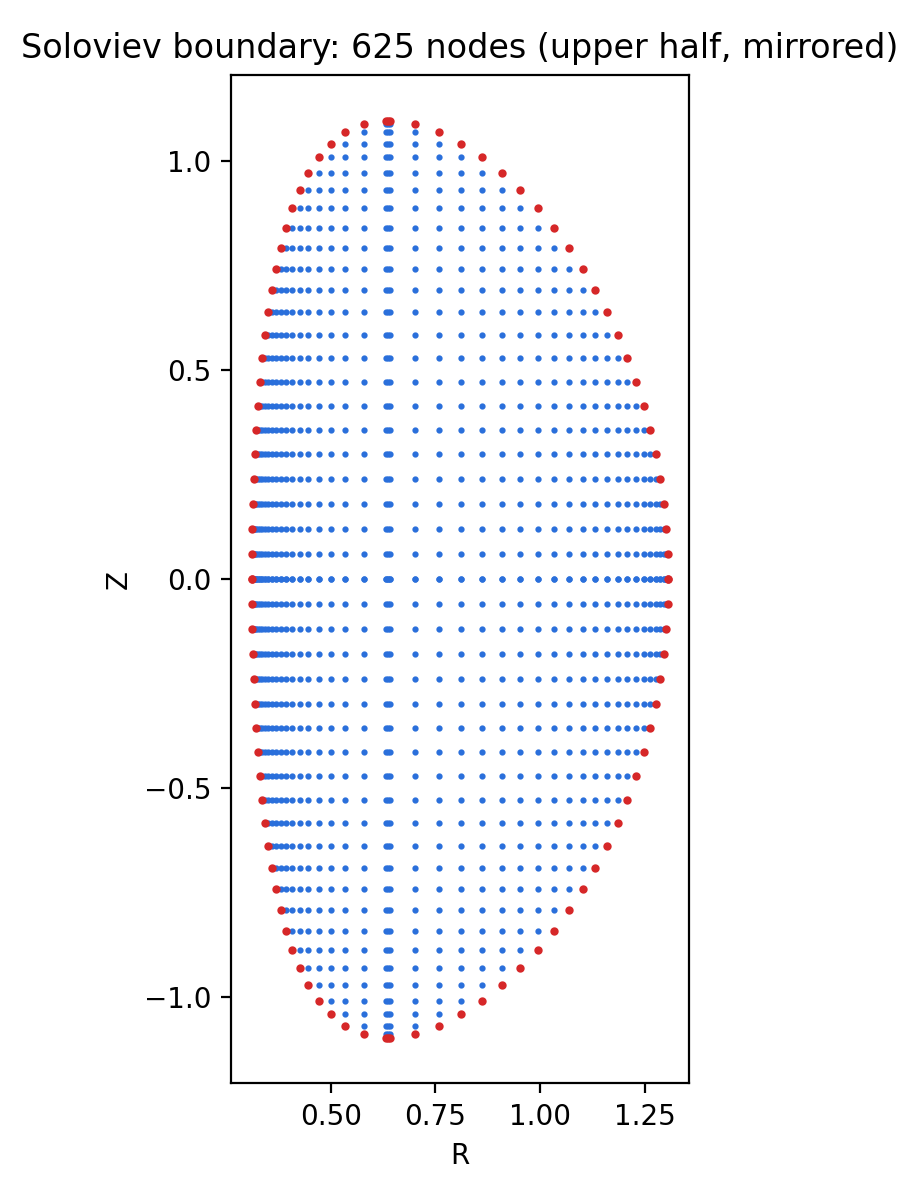
\includegraphics[height=6.2cm]{mesh_soloviev.png}\hspace{1cm}
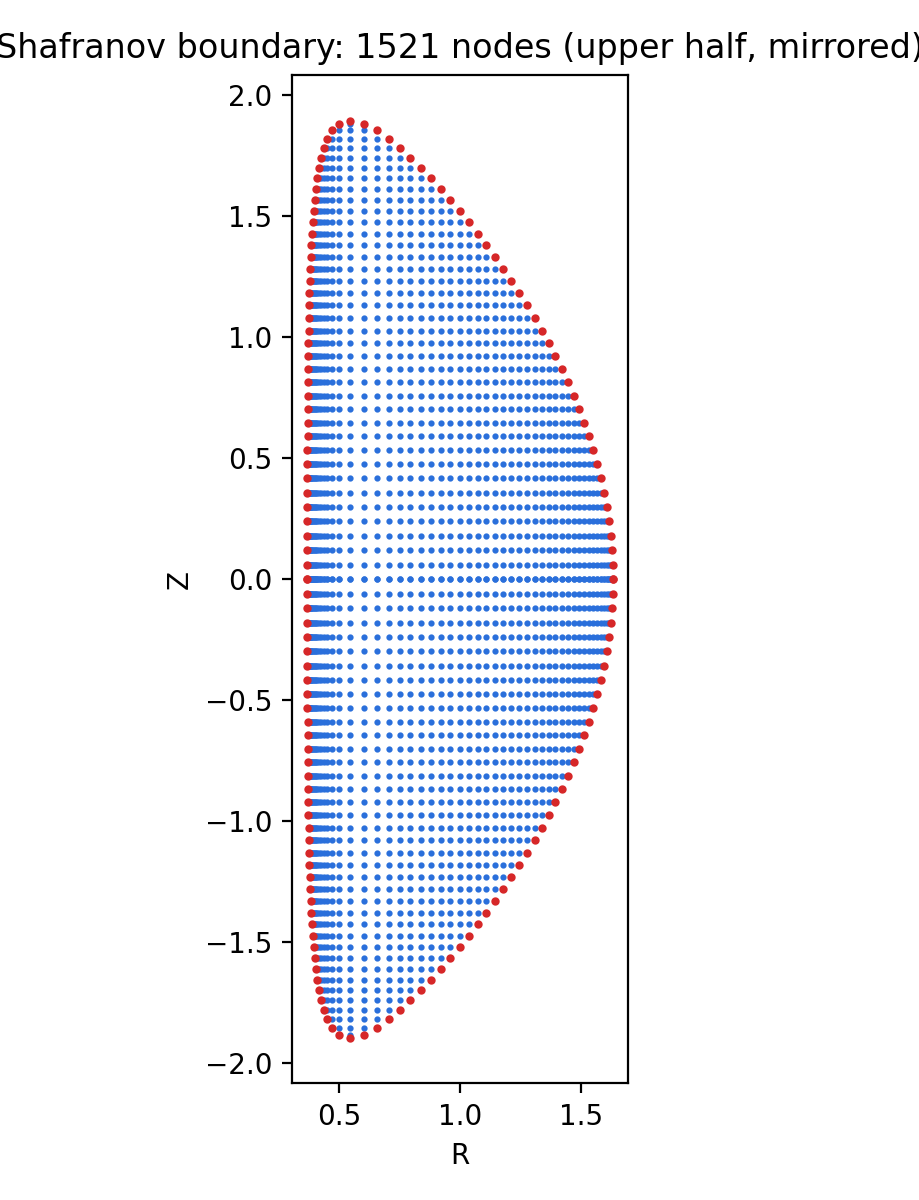
\includegraphics[height=6.2cm]{mesh_shafranov.png}
\caption{Non-homogeneous boundary-fitted meshes (upper half computed, mirrored for display). Red: Dirichlet nodes, blue: interior nodes. Left: Solov'ev contour; right: Shafranov parametric boundary ($\kappa=3$, $\delta=0.8$).}
\label{fig:mesh}
\end{figure}

\subsection{Finite-difference discretisation}
On a non-uniform 3-point stencil with $h_+=x_{i+1}-x_i$, $h_-=x_i-x_{i-1}$ and $h_s=h_++h_-$, the second-order accurate approximations are
\begin{align}
f''_i&\approx\frac{2}{h_s}\left[\frac{f_{i+1}-f_i}{h_+}+\frac{f_{i-1}-f_i}{h_-}\right],\\
f'_i&\approx\frac{h_-^2\,(f_{i+1}-f_i)-h_+^2\,(f_{i-1}-f_i)}{h_+h_-h_s}.
\end{align}
(The leading truncation error of the first-derivative formula is $\tfrac16h_+h_-f'''$, so it is second order in the local mesh size; the second-derivative formula is first order at nodes with $h_+\neq h_-$ and second order on smoothly graded meshes, which is the case here.) Applying these in $r$ for $\partial_r^2-\tfrac1r\partial_r$ and in $z$ for $\partial_z^2$ gives, at an interior node $(i,j)$ with $r=r_i$,
\begin{equation}
\Dstar\psi\big|_{ij}\approx c_{R+}\psi_{i+1,j}+c_{R-}\psi_{i-1,j}+c_{Z+}\psi_{i,j+1}+c_{Z-}\psi_{i,j-1}+c_0\psi_{ij},
\end{equation}
with, in terms of $h_\pm^{(r)}$, $h_s^{(r)}$ and $h_\pm^{(z)}$, $h_s^{(z)}$,
\begin{align*}
c_{R+}&=\frac{2}{h^{(r)}_+h^{(r)}_s}-\frac{(h^{(r)}_-)^2}{r\,h^{(r)}_+h^{(r)}_-h^{(r)}_s}, &
c_{R-}&=\frac{2}{h^{(r)}_-h^{(r)}_s}+\frac{(h^{(r)}_+)^2}{r\,h^{(r)}_+h^{(r)}_-h^{(r)}_s},\\
c_{Z\pm}&=\frac{2}{h^{(z)}_\pm h^{(z)}_s}, &
c_0&=-\frac{2}{h^{(r)}_+h^{(r)}_-}+\frac{(h^{(r)}_-)^2-(h^{(r)}_+)^2}{r\,h^{(r)}_+h^{(r)}_-h^{(r)}_s}-\frac{2}{h^{(z)}_+h^{(z)}_-}.
\end{align*}
This is the same structure as L\'opez's Eq.~(14), written for the operator in the form used in this code.

\paragraph{Boundary conditions.}
\begin{itemize}[nosep]
\item \emph{Midplane} ($z=0$, symmetry): a ghost value $\psi_{i,-1}=\psi_{i,1}$ gives $\partial_z^2\psi|_{z=0}\approx 2(\psi_{i,1}-\psi_{i,0})/(h^{(z)}_+)^2$.
\item \emph{Boundary}: a node is \emph{Dirichlet} ($\psi=\psi_b$, which is $1$ in normalised units) if it is on the top row, or has a missing active neighbour in the $r$-direction (inner/outer wall), or a missing neighbour in $z$ (except at the midplane, where the ghost value is used). Dirichlet rows of the matrix are identity rows. Because the grid lines pass through the boundary points in $R$, the radial condition is imposed exactly; a node whose vertical neighbour is missing is, however, assigned the boundary value even though it lies slightly inside the boundary in $z$, which is the main source of the discretisation error discussed in Section~\ref{sec:bench}.
\end{itemize}

\subsection{Sparse linear algebra}
Collecting the active nodes in a single index $k$ gives a linear system $A\bm\psi=\bm b$, where $A\in\mathbb R^{N\times N}$ has at most five non-zeros per row. It is assembled in LIL format (cheap incremental insertion), converted to CSR, and solved with \texttt{scipy.sparse.linalg.spsolve} (sparse LU, SuperLU). Dirichlet rows read $\psi_k=1$ with $b_k=1$; interior rows read $(A\bm\psi)_k=S_k$. For Solov'ev, a single solve ($\approx 0.1$\,s for $N\approx6000$) is enough. The matrix does \emph{not} depend on $\bm\psi$ in the nonlinear case, only the right-hand side does; the present code nevertheless refactorises at each Picard step, so an easy speed-up is to compute one \texttt{splu} factorisation and reuse it.

\subsection{Picard iteration for the nonlinear case}\label{sec:picarddef}
For the nonlinear source, one step of the iteration is a map $P:\bm\psi\mapsto\bm\psi^{+}$ defined as
\begin{enumerate}[nosep]
\item compute the normalised flux $\pn=(\psi-\psi_{\min})/(\bar\psi_b-\psi_{\min})$ at every node, clipped to $[0,1]$ ($\psi_{\min}$ is the minimum over the grid, $\bar\psi_b$ the mean boundary value);
\item evaluate the right-hand side $b_k=S(r_k,\pn^{(k)})$ at interior nodes ($b_k=1$ on the boundary);
\item solve $A\bm u=\bm b$;
\item renormalise $\bm\psi^+=(\bm u-u_{\min})/(\bar u_b-u_{\min})$.
\end{enumerate}
The iteration (a plain fixed-point or Picard iteration on the nonlinear source, see e.g.\ Jardin~\cite{jardin2010}) is started from $\psi=0$ in the interior and $\psi=1$ on the boundary, $\bm\psi^{k+1}=P(\bm\psi^k)$. A solution of the normalised GS problem is a fixed point $P(\bm\psi)=\bm\psi$, so the stopping test is the \emph{fixed-point residual} $\|P(\bm\psi)-\bm\psi\|/\|\bm\psi\|<10^{-9}$; for every nonlinear run the code reports it, together with $\|P(P(\bm\psi))-\bm\psi\|/\|\bm\psi\|$, and prints a warning if $\bm\psi$ is not a fixed point (and if the iteration looks like a period-two cycle). 
Two structural remarks:
\begin{itemize}[nosep]
\item Because $A$ is linear and step~4 removes any overall factor, \emph{only the ratio $p_0/\alpha$ matters} for the normalised map: scaling $(p_0,\alpha)\to s\,(p_0,\alpha)$ scales $\bm u-\bm 1$ by $s$, which the renormalisation undoes.
\item L\'opez \emph{et al.}\ instead hold the total plasma current and the on-axis pressure fixed by adjusting a coefficient in the $f^2$ profile at every iteration (their Eqs.~(15)--(17)); the code here does not implement that constraint.
\end{itemize}
The geometry is validated at start-up: the Shafranov boundary requires $a<R_0$, since otherwise the plasma crosses $R=0$ where the $1/R$ term of $\Dstar$ is singular.

%=====================================================================
\section{Results}\label{sec:results}
%=====================================================================

\subsection{Benchmark against the Solov'ev solution}\label{sec:bench}
We use the parameters of~\cite{lopez2019}: $B_0=0.5$\,T, $R_0=0.95$, $\kappa_0=2.2$, $q_0=1.1$, $\psi_b=0.09$, on the Solov'ev contour, in mode \texttt{SOLOVIEV\_LINEAR}. Figure~\ref{fig:soloviev} shows the numerical and exact fluxes and their difference for $\Delta s=0.02$ ($N=5041$ unknowns, a $141\times71$ tensor grid of which every active node is used): the maximum error is $1.9\times10^{-5}$ and the mean error $4.7\times10^{-6}$, i.e.\ $2\times10^{-4}$ relative to the peak value of $\psi$. The error is largest around the magnetic axis and decays towards the boundary, where $\psi$ is prescribed.

\begin{figure}[t]
\centering
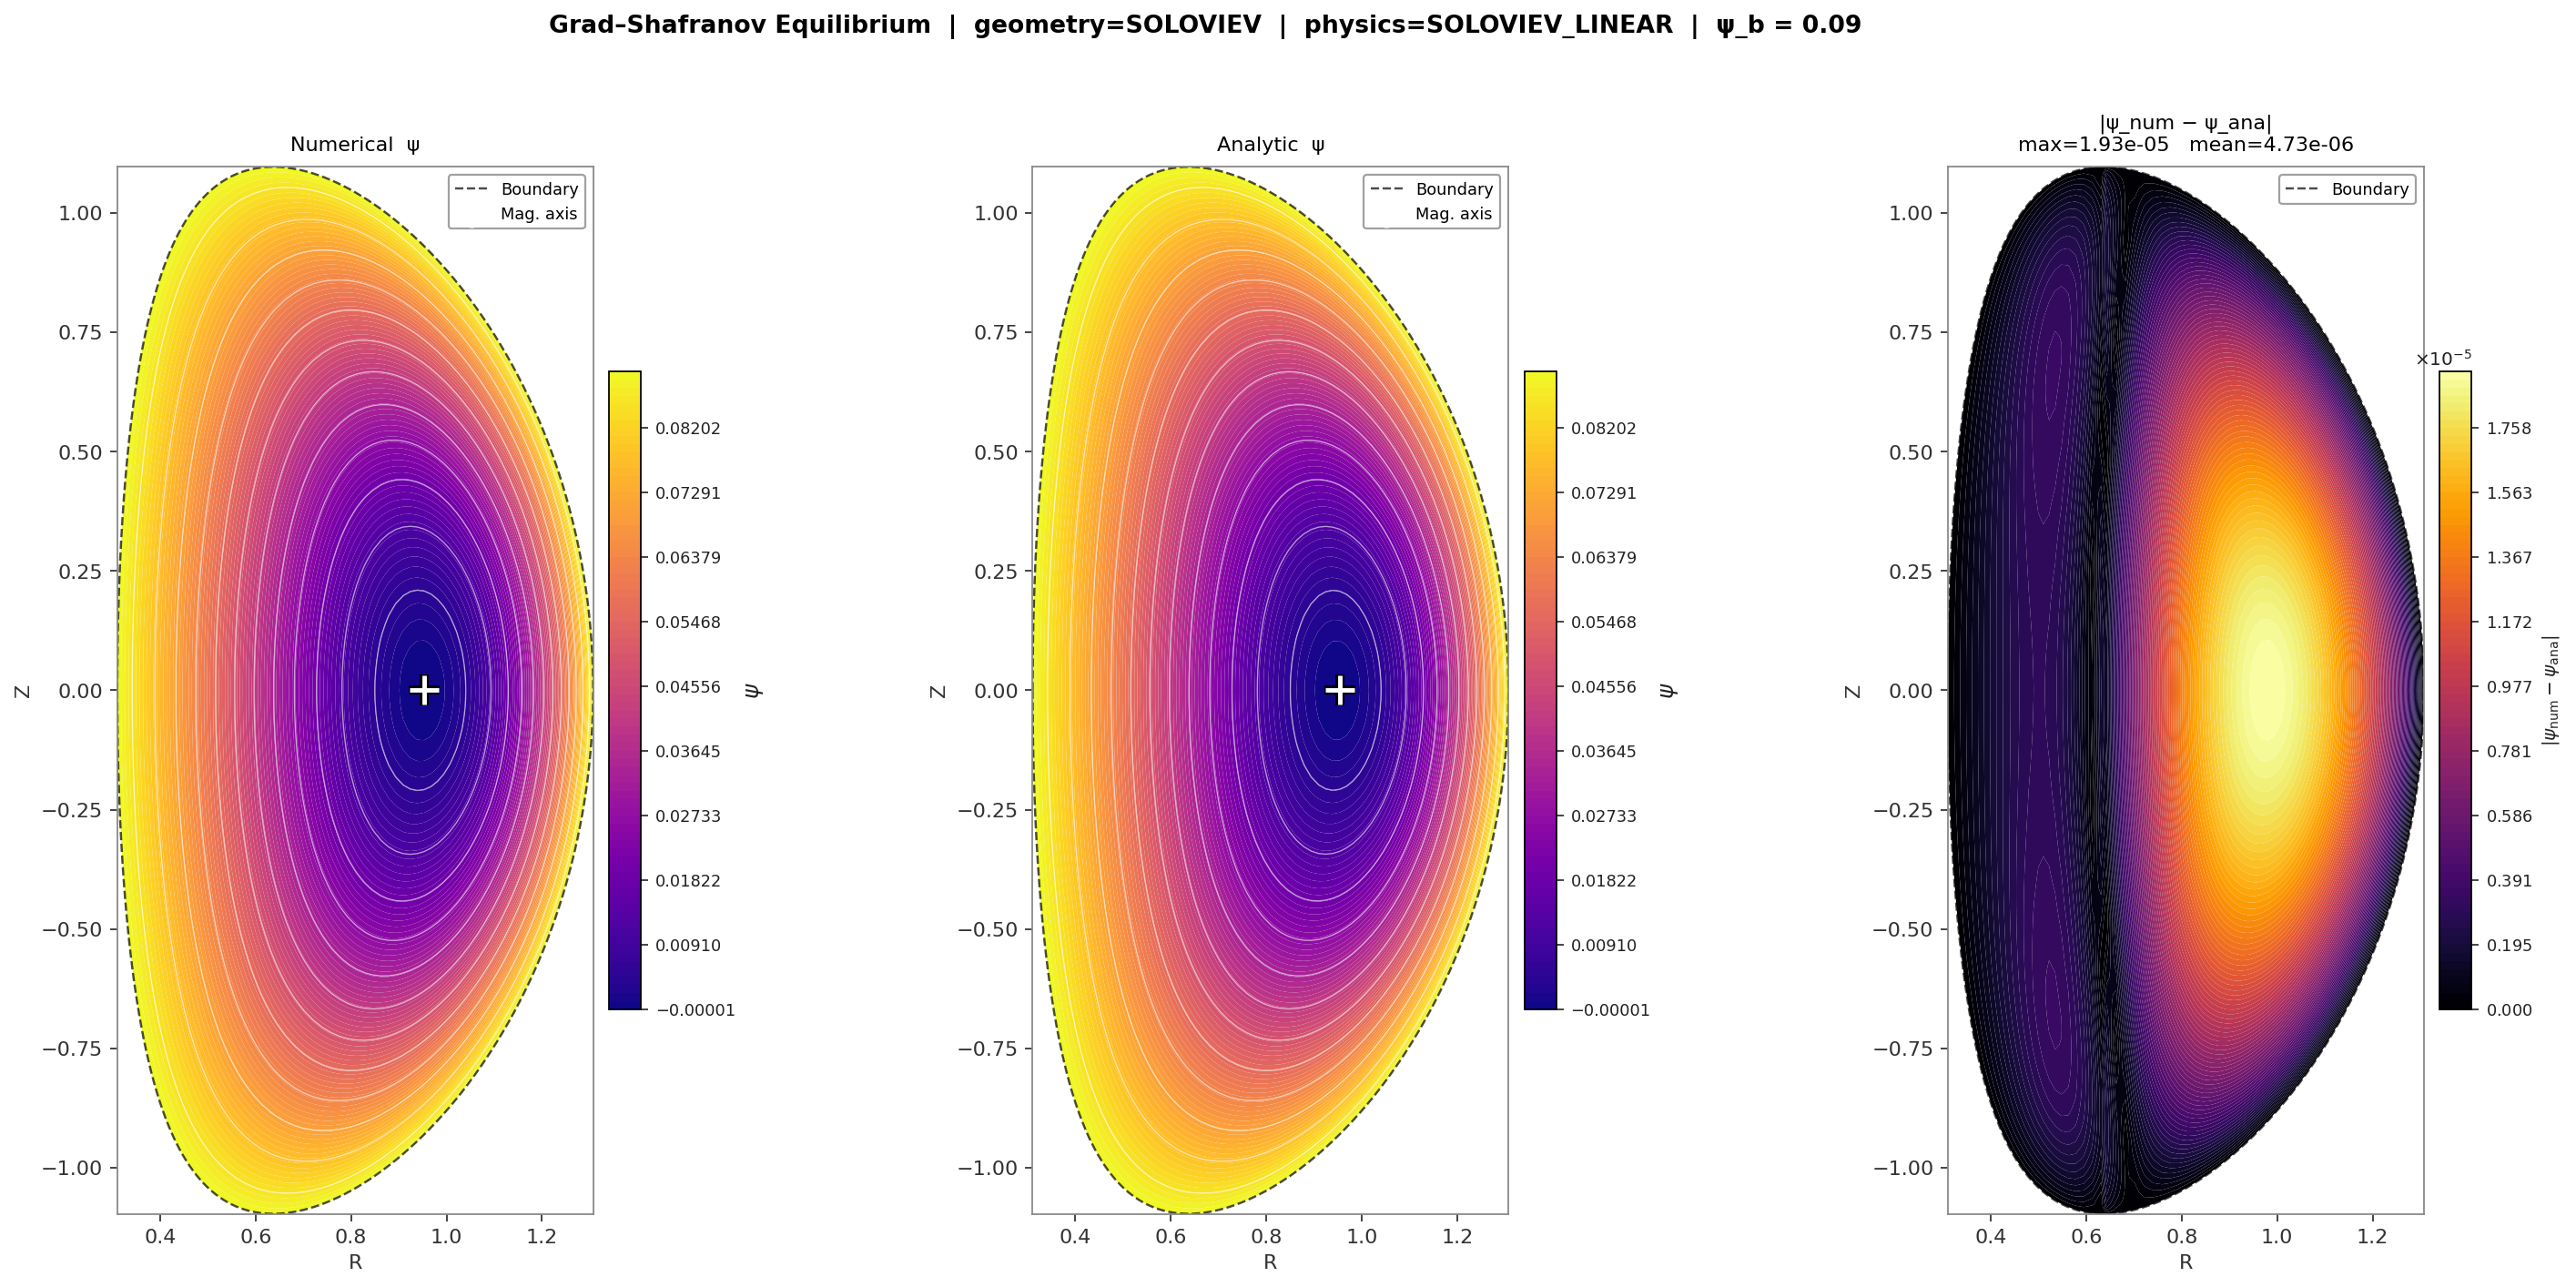
\includegraphics[width=\textwidth]{soloviev_benchmark.png}
\caption{Linear Solov'ev benchmark, $\Delta s=0.02$. Left: numerical $\psi$; middle: analytic $\psi$; right: absolute error.}
\label{fig:soloviev}
\end{figure}

\paragraph{Grid convergence.}
Table~\ref{tab:conv} and Figure~\ref{fig:conv} show the error as the boundary step $\Delta s$ is refined. A least-squares fit on the log--log data gives an observed order of $1.88$ (max norm) and $1.79$ (mean), i.e.\ close to the second order expected for the stencils. The slightly sub-quadratic max-norm slope is consistent with the first-order treatment of the vertical boundary condition noted above. For reference, L\'opez \emph{et al.} report on a $241\times241$ mesh an error along the $r$ axis that does not exceed $10^{-5}$ (their Fig.~4c). Our run at $\Delta s=0.012$ ($233\times233$ tensor grid, $N=13689$ active nodes) has a maximum error of $7.0\times10^{-6}$ over the whole grid, which is of the same order and slightly below that bound at comparable resolution; we have not reproduced their SOR iteration and the comparison is only as precise as their one-line statement.

\begin{table}[h]
\centering
\caption{Solov'ev grid-convergence study (error in $\psi$ in the units of $\psi_b=0.09$).}
\label{tab:conv}
\begin{tabular}{rrcc}
\toprule
$\Delta s$ & $N$ & max error & mean error\\
\midrule
0.200 & 81   & $1.34\times10^{-3}$ & $2.65\times10^{-4}$\\
0.140 & 144  & $7.34\times10^{-4}$ & $1.45\times10^{-4}$\\
0.100 & 256  & $4.08\times10^{-4}$ & $8.40\times10^{-5}$\\
0.070 & 441  & $2.14\times10^{-4}$ & $4.94\times10^{-5}$\\
0.050 & 841  & $1.11\times10^{-4}$ & $2.61\times10^{-5}$\\
0.035 & 1681 & $5.59\times10^{-5}$ & $1.33\times10^{-5}$\\
0.025 & 3249 & $2.94\times10^{-5}$ & $7.14\times10^{-6}$\\
0.018 & 6241 & $1.53\times10^{-5}$ & $3.72\times10^{-6}$\\
0.012 & 13689 & $6.99\times10^{-6}$ & $1.74\times10^{-6}$\\
\bottomrule
\end{tabular}
\end{table}

\begin{figure}[h]
\centering
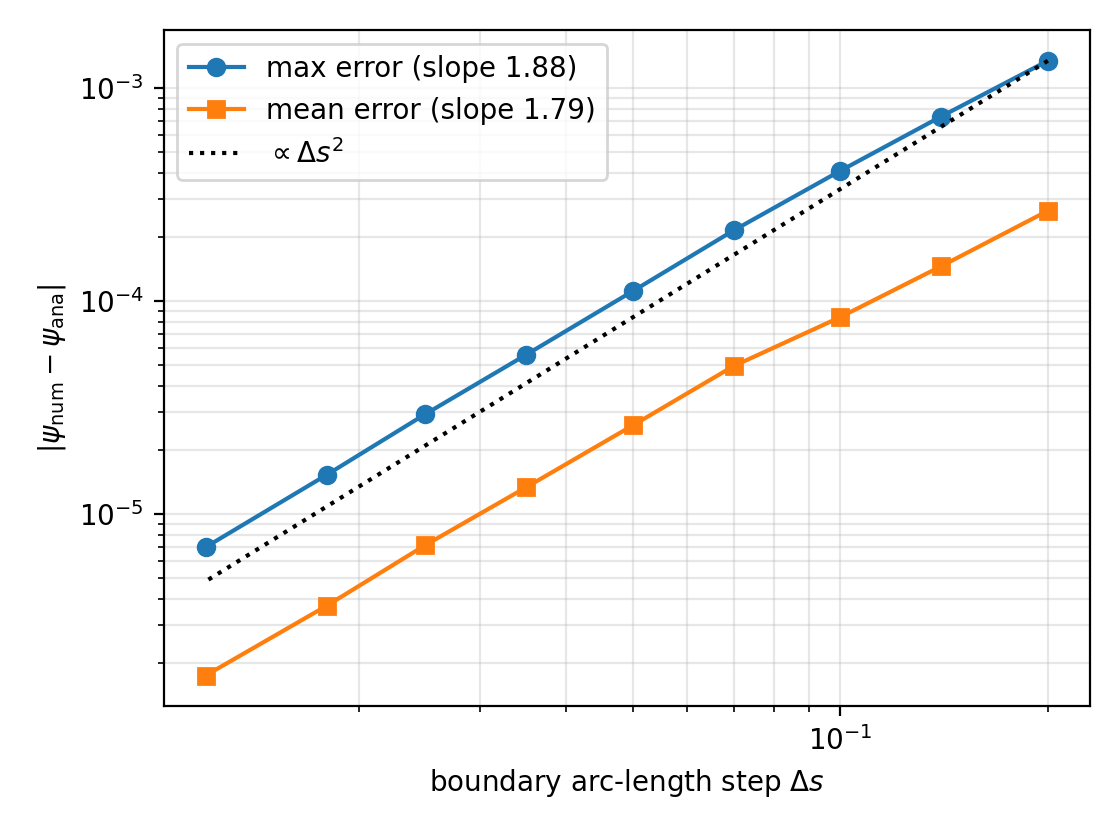
\includegraphics[width=0.55\textwidth]{soloviev_convergence.png}
\caption{Error versus boundary step; dotted: $\propto\Delta s^2$.}
\label{fig:conv}
\end{figure}

\subsection{Validation of the nonlinear code path}\label{sec:nlval}
There is no analytic solution for a generic nonlinear source, so the nonlinear path is validated in two ways (\texttt{scripts/nonlinear\_validation.py}).
\paragraph{Solov'ev through the Picard path.} Running the Picard machinery (\texttt{CUSTOM} source equal to the exact Solov'ev source, plain iteration) must reproduce the analytic solution. It does, converging in 2 iterations (one solve plus one confirming step) to a residual below $10^{-12}$, with maximum errors from $5\times10^{-4}$ at $N=144$ down to $1.7\times10^{-5}$ at $N=3249$, an observed order of $1.9$. The errors are not strictly monotone because the renormalisation uses the discrete minimum of $\psi$, which exceeds the true axis value by an amount that varies with the (non-nested) mesh.
\paragraph{Grid convergence of a nonlinear case.} For the ITER-like boundary with baseline profiles we track the amplitude functional $C=1-u_{\min}$ (the flux difference between boundary and axis in the unnormalised solve at the fixed point) for $N=144$ up to $6889$. It converges, from $0.16780$ to $0.16729$, with a fit $C(\Delta s)=C_\infty+c\,\Delta s^{p}$ giving $C_\infty=0.16723$ and $p\approx1.2$; the plain iteration needs $27$--$28$ iterations at every resolution and the residual is $<4\times10^{-13}$ throughout. The observed order is closer to one than to two, consistent with the first-order treatment of the vertical boundary condition and with non-nested meshes. We therefore claim convergence, but not second-order accuracy, for the nonlinear solutions.

\subsection{Nonlinear equilibria: profiles and shapes}\label{sec:profiles}
We use the Shafranov boundary with $R_0=0.95$, $a=0.6$ ($a/R_0=0.63$), $\Delta s=0.05$, and plain Picard iteration. Baseline exponents are $(s_{p1},s_{p2})=(2,2)$, $(s_{f1},s_{f2})=(2,1)$ and $p_0=\alpha=1$. We first vary the boundary shape, then the profiles at the ITER-like shape $\kappa=1.7$, $\delta=0.33$. Table~\ref{tab:nl} lists the iterations needed, the fixed-point residual, the position of the magnetic axis (parabolic interpolation through the three midplane nodes around the minimum) and its displacement from the geometric centre of the midplane chord, normalised by the half-width of that chord.

\begin{table}[h]
\centering
\caption{Nonlinear cases (plain Picard). All reach a true fixed point of $P$.}
\label{tab:nl}
\small
\begin{tabular}{llrrcccc}
\toprule
case & $(\kappa,\delta)$ & $N$ & iter. & $\|P\bm\psi-\bm\psi\|/\|\bm\psi\|$ & $R_{\rm axis}$ & shift/half-width\\
\midrule
circular                          & (1.0, 0.00) & 441  & 22 & $1.9\times10^{-11}$ & 1.174 & $+0.275$\\
ITER-like (baseline)              & (1.7, 0.33) & 961  & 23 & $1.6\times10^{-11}$ & 1.152 & $+0.240$\\
strong D                          & (3.0, 0.80) & 2209 & 30 & $2.6\times10^{-11}$ & 1.151 & $+0.238$\\
\midrule
peaked $p'$, $(s_{p1},s_{p2})=(2,4)$      & (1.7, 0.33) & 961 & 26 & $2.3\times10^{-11}$ & 1.149 & $+0.236$\\
broad $p'$, $FF'$, $(4,1)$ and $(4,1)$    & (1.7, 0.33) & 961 & 15 & $1.3\times10^{-11}$ & 1.147 & $+0.232$\\
current-driven, $p_0{=}0.2,\ \alpha{=}2$  & (1.7, 0.33) & 961 & 20 & $1.4\times10^{-11}$ & 1.078 & $+0.124$\\
pressure-driven, $p_0{=}3,\ \alpha{=}0.3$ & (1.7, 0.33) & 961 & 25 & $3.7\times10^{-11}$ & 1.189 & $+0.300$\\
\bottomrule
\end{tabular}
\end{table}

\begin{figure}[t]
\centering
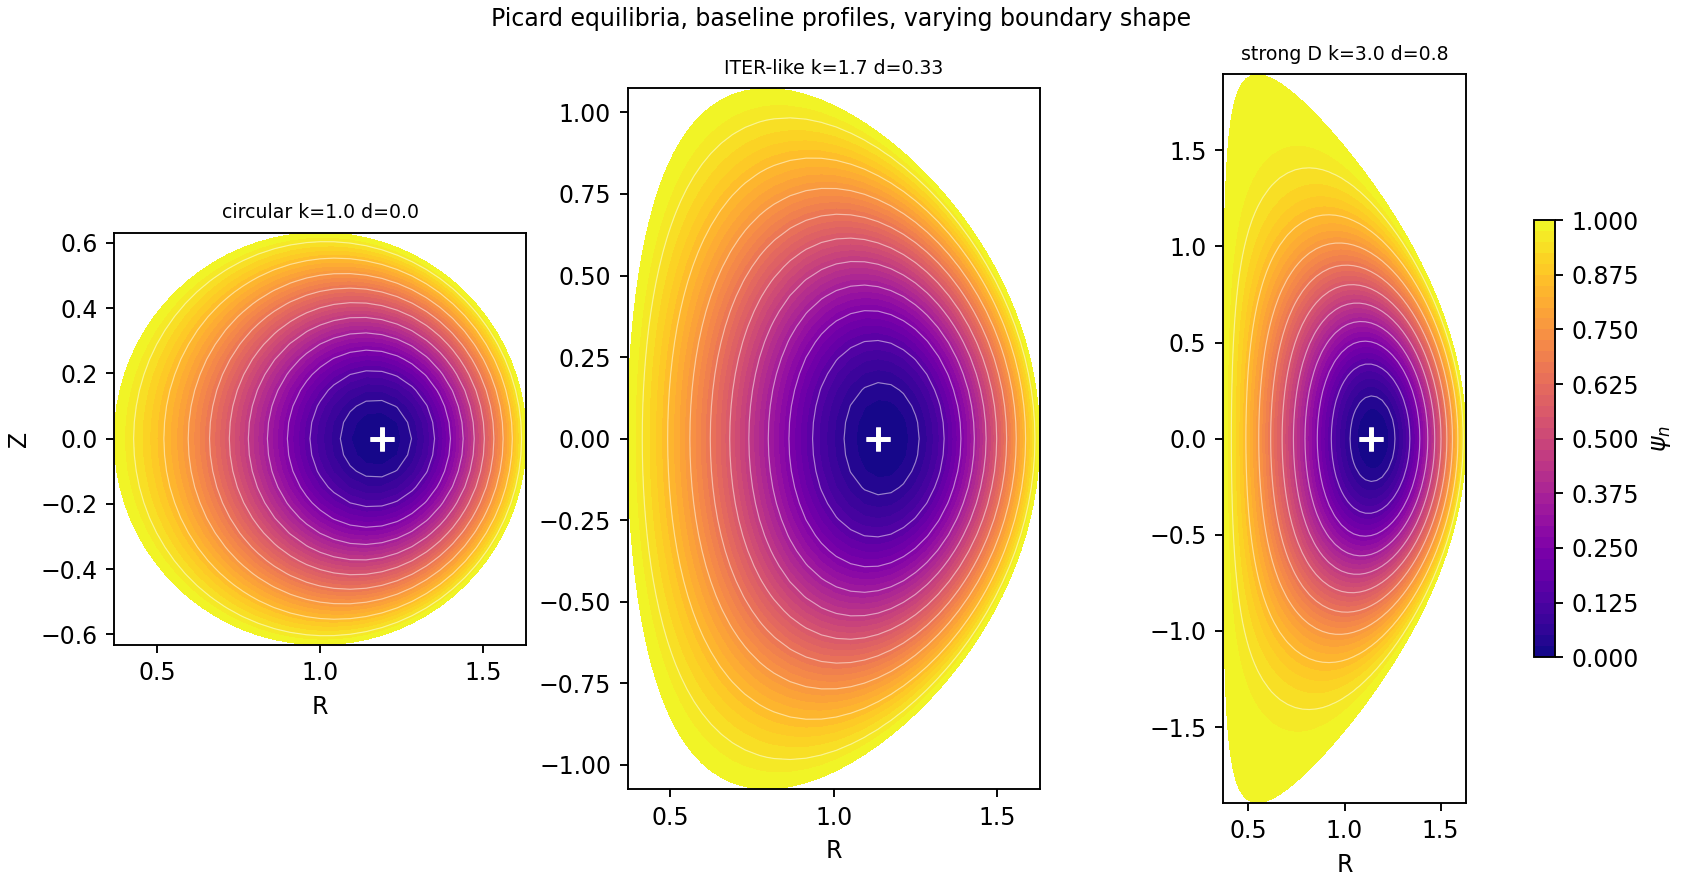
\includegraphics[width=\textwidth]{nonlinear_shapes.png}
\caption{Flux surfaces ($\pn$ contours; white $+$: magnetic axis) at the baseline profiles for three boundary shapes: circular, ITER-like, strong D.}
\label{fig:shapes}
\end{figure}

\begin{figure}[t]
\centering
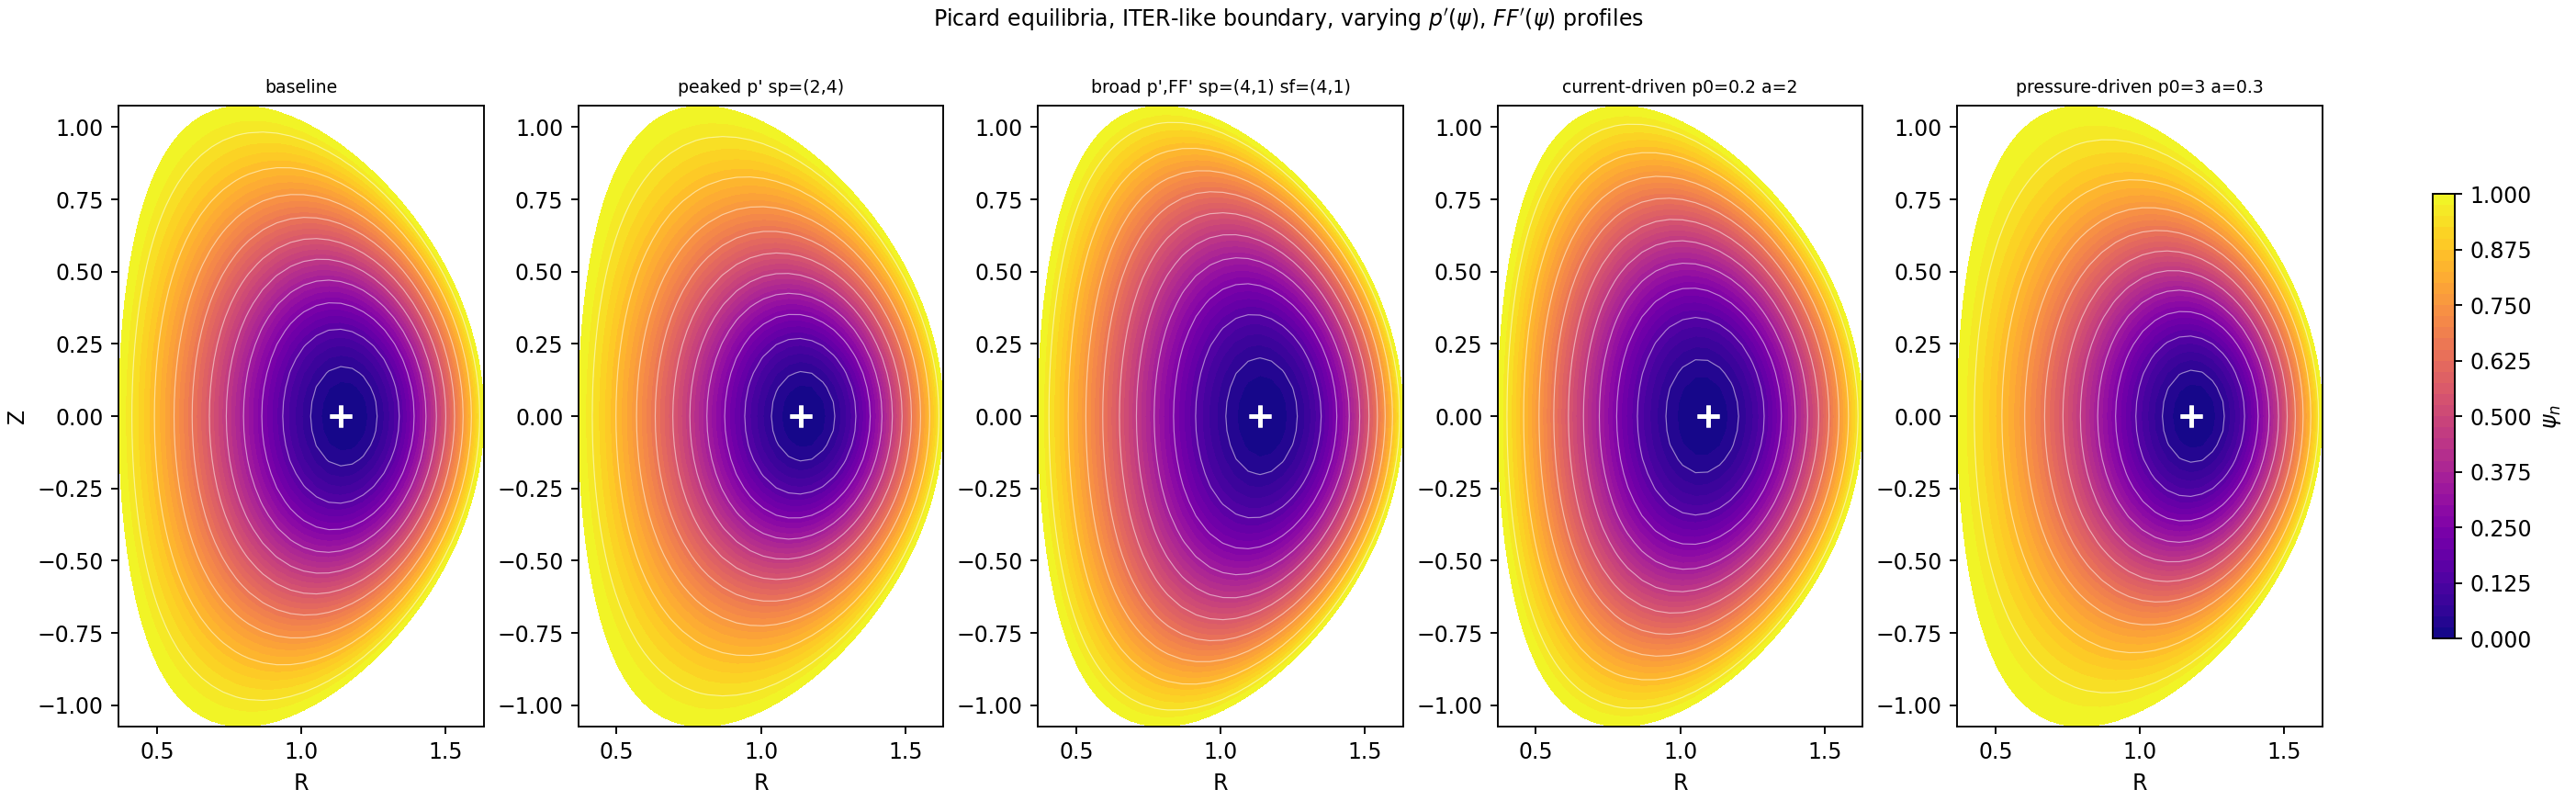
\includegraphics[width=\textwidth]{nonlinear_profiles.png}
\caption{Flux surfaces at the ITER-like boundary for five choices of the profiles.}
\label{fig:profiles}
\end{figure}

\begin{figure}[t]
\centering
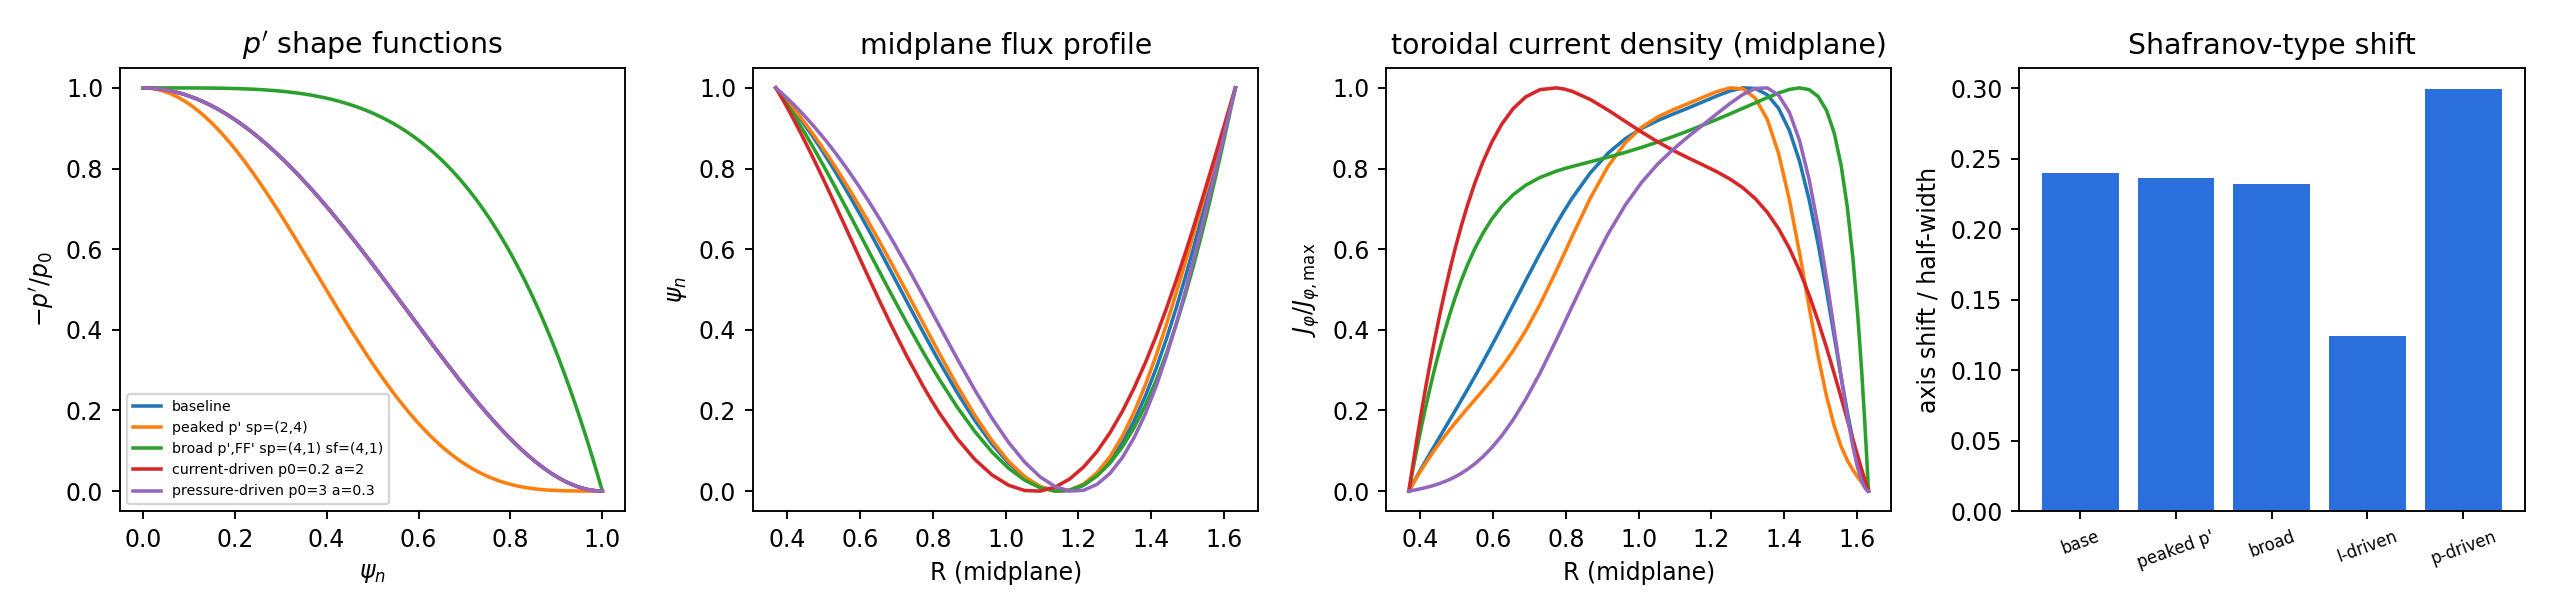
\includegraphics[width=\textwidth]{nonlinear_profile_diagnostics.png}
\caption{Left to right: shape of $-p'$; midplane flux profile; midplane toroidal current density $J_\varphi\propto S/R$ (each case normalised to its maximum); normalised axis shift.}
\label{fig:diag}
\end{figure}

\paragraph{What the cases show.}
\begin{itemize}[nosep]
\item \emph{Toroidicity shifts the axis outward even for a circular boundary.} The circular case is not symmetric under $R\to2R_0-R$ (the operator contains $1/R$), and the axis sits at $+0.28$ half-widths outward of the geometric centre. This is the Shafranov shift: the flux surfaces are compressed on the outboard side and the axis moves outward relative to the centre of the boundary. Increasing the shaping to $\kappa=1.7,\delta=0.33$ or to $\kappa=3,\delta=0.8$ changes the normalised shift only slightly ($0.275\to0.240\to0.238$), while the surfaces follow the D-shape (Fig.~\ref{fig:shapes}).
\item \emph{The shift is controlled by the pressure-to-current ratio, not by the peaking of $p'$.} At fixed ratio $p_0/\alpha=1$, changing the exponents (peaked, baseline or broad $p'$ and $FF'$) moves the shift only between $0.232$ and $0.240$. In contrast, the ratio does the work: $p_0/\alpha=0.1$ gives $0.124$ and $p_0/\alpha=10$ gives $0.300$, a factor $2.4$. This is consistent with the dependence of the Shafranov shift on poloidal beta: more pressure support relative to the poloidal-field-producing current pushes the axis outward.
\item \emph{The current density profile follows suit.} Because $J_\varphi\propto S/R$ and the pressure term of $S$ carries a factor $R^2$, the midplane current density peaks outboard of the axis for pressure-driven profiles and inboard for current-driven ones (Fig.~\ref{fig:diag}, third panel), but it never vanishes on the axis.
\item \emph{Cost.} All cases converge to residuals of $10^{-11}$ in $15$--$30$ plain Picard iterations; broader profiles converge fastest (spectral radius $0.22$ versus $0.44$ for the peaked $p'$; Table~\ref{tab:spec}).
\end{itemize}

%=====================================================================
\section{Convergence of the Picard iteration}\label{sec:picard}
%=====================================================================

\subsection{Linear stability}
Let $P$ be the one-step Picard map of Section~\ref{sec:picarddef}, $\bm\psi^*$ a fixed point and $L=\partial P/\partial\bm\psi|_{\bm\psi^*}$ its Jacobian. Near $\bm\psi^*$ the error evolves as $\bm e^{k+1}\approx L\bm e^k$, so plain Picard converges if and only if the spectral radius $\rho(L)<1$, with asymptotic rate $\rho(L)$ per iteration; reducing the residual by a factor $\varepsilon$ takes about $\ln\varepsilon/\ln\rho(L)$ iterations. We build $L$ column by column by central differences, $L\bm e_j\approx[P(\bm\psi^*+\eta\bm e_j)-P(\bm\psi^*-\eta\bm e_j)]/2\eta$ with $\eta=10^{-6}\|\bm\psi^*\|$, and diagonalise it densely (grids up to $N\approx10^3$). For larger grids the code can instead estimate the leading eigenvalues matrix-free with \texttt{scipy.sparse.linalg.eigs} (\texttt{SPECTRAL\_ANALYSIS}).

\subsection{Measurements}
All numbers below come from \texttt{scripts/spectral\_study.py} (output in \texttt{results/spectral\_study.json}).

\begin{figure}[t]
\centering
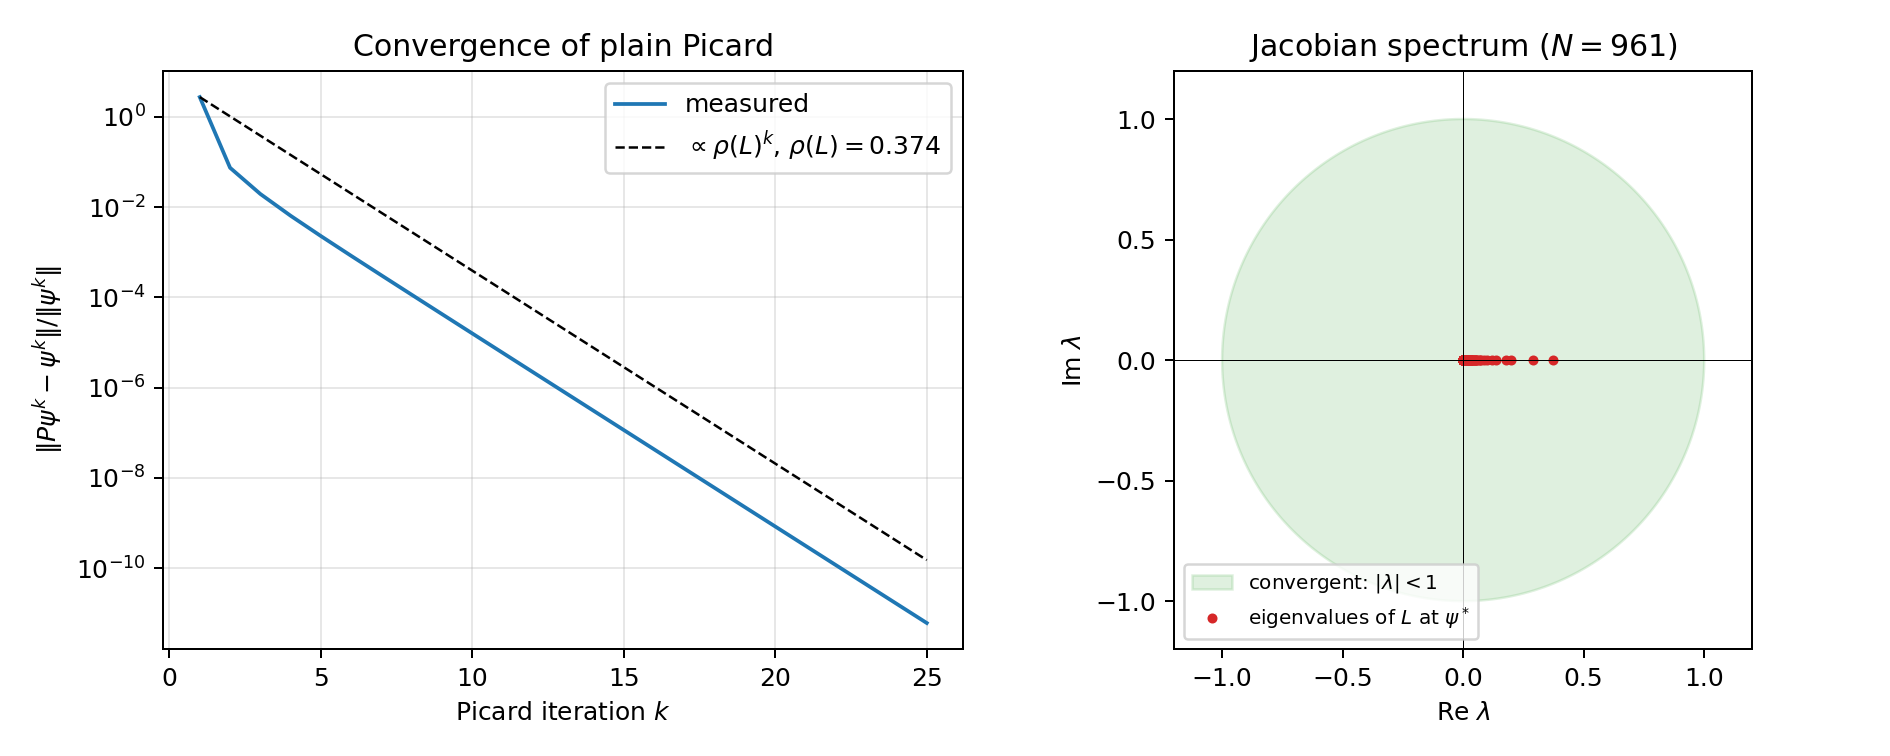
\includegraphics[width=\textwidth]{picard_spectral_study.png}
\caption{Left: fixed-point residual of plain Picard (ITER-like boundary, baseline profiles, $N=961$) and the decay $\rho(L)^k$ predicted by the spectral radius. Right: eigenvalues of the Picard Jacobian $L$ at the fixed point against the unit disc.}
\label{fig:spectral}
\end{figure}

\paragraph{Main case ($N=961$).} Plain Picard reaches a residual of $10^{-11}$ in $25$ iterations. The spectrum of $L$ at the fixed point is real and non-negative, $\lambda\in[0,0.374]$ (largest imaginary part $2\times10^{-6}$), so $\rho(L)=0.374$ and the predicted number of iterations is $\ln10^{-11}/\ln0.374=25.7$, matching the observed $25$ (Fig.~\ref{fig:spectral}).

\begin{table}[h]
\centering
\caption{Plain-Picard iterations (to a residual of $10^{-11}$) and spectral radius of $L$ at the fixed point, dense Jacobian. In every case the spectrum is real and non-negative to within $4\times10^{-4}$ in imaginary part.}
\label{tab:spec}
\small
\begin{tabular}{lrcc}
\toprule
case & $N$ & iterations & $\rho(L)$\\
\midrule
ITER-like, baseline              & 484 & 25 & 0.380\\
circular                         & 225 & 24 & 0.374\\
strong D $(3.0,0.8)$             & 576 & 33 & 0.484\\
pressure-driven, $p_0/\alpha=10$ & 484 & 28 & 0.420\\
current-driven, $p_0/\alpha=0.1$ & 484 & 22 & 0.316\\
broad profiles                   & 484 & 17 & 0.219\\
peaked $p'$                      & 484 & 29 & 0.437\\
\bottomrule
\end{tabular}
\end{table}

\paragraph{Reading.} With peaked-current profiles the Jacobian has a real, non-negative spectrum inside $[0,0.5)$, so plain Picard converges monotonically with rate $0.22$--$0.48$ in all seven configurations tested, and $\rho(L)$ predicts the iteration count well. Broader profiles converge fastest; strong shaping and peaked $p'$ slowest. We have not tested hollow-current, high-beta or very strongly shaped profiles, where the spectrum could look different.

\subsection{Profile parametrisation: why the shapes are on $p'$ and $FF'$}\label{sec:param}
\texttt{scripts/profile\_parametrisation\_check.py} runs plain Picard on the ITER-like boundary for sources built in different ways (Table~\ref{tab:param}). When the shapes $(1-\pn^{2})^{2}$ are imposed on $p$ and $F^2$ and then differentiated, the derivatives are proportional to $\pn$ and vanish on the axis: $S(\pn=0)=0$ and $J_\varphi=0$ on the magnetic axis (a hollow current). In that case plain Picard does not converge: after $800$ iterations $\|P\bm\psi-\bm\psi\|/\|\bm\psi\|\approx0.11$--$0.12$ while $\|P(P\bm\psi)-\bm\psi\|\sim10^{-12}$, i.e.\ the iterates oscillate between two states, a period-two cycle of $P$. This residual is the same at $\Delta s=0.10,0.05$ and $0.035$, so it is not a resolution effect. With exponents $(1,1,1)$ (source independent of $\psi$) or $(1,2,1)$ (nonzero $p'$ on the axis, source depends on $\psi$) the same code converges to residuals of $10^{-11}$--$10^{-13}$, as does the default derivative-shaped source.

\begin{table}[h]
\centering
\caption{Plain Picard (up to 800 iterations) for different ways of imposing the profile shapes ($\Delta s=0.05$; the other resolutions are in \texttt{results/profile\_parametrisation\_check.json}).}
\label{tab:param}
\small
\begin{tabular}{lccc}
\toprule
shape imposed on & iterations & $\|P\bm\psi-\bm\psi\|/\|\bm\psi\|$ & $\|P^2\bm\psi-\bm\psi\|/\|\bm\psi\|$\\
\midrule
$p'$, $FF'$ (default)             & 23  & $1.6\times10^{-11}$ & $2.2\times10^{-11}$\\
$p$, $F^2$, exponents $(2,2,2)$   & 800 & $1.1\times10^{-1}$  & $3.8\times10^{-13}$\\
$p$, $F^2$, exponents $(1,1,1)$   & 2   & $5\times10^{-14}$   & $7\times10^{-14}$\\
$p$, $F^2$, exponents $(1,2,1)$   & 15  & $1.1\times10^{-11}$ & $1.4\times10^{-11}$\\
\bottomrule
\end{tabular}
\end{table}

We have not proved \emph{why} a vanishing source on the axis produces the oscillation; the evidence is this controlled comparison. The practical rule is to impose the profile shapes on $p'$ and $FF'$ for peaked-current equilibria, and to use the fixed-point residual, not the size of the last step, to decide whether a nonlinear run has produced a solution.

\subsection{Outlook}
\begin{itemize}[nosep]
\item Implement the constraint of L\'opez \emph{et al.}\ (fixed total current and axis pressure via a coefficient adjusted each iteration), and compare.
\item Reuse one sparse LU factorisation across Picard iterations, since $A$ does not change.
\item A free-boundary variant on top of the same matrix machinery; inverse reconstruction of $p'$, $FF'$ from synthetic data.
\item Quantitative checks of the nonlinear solutions against a published nonlinear equilibrium, which this work does not provide.
\end{itemize}

%=====================================================================
\appendix
\section{Derivation of the Grad--Shafranov equation}\label{app:derivation}
%=====================================================================
\emph{This derivation follows the approach of Ben Dudson's lecture series ``Plasma fluid theory''~\cite{dudson}.} The three ingredients are $\bB=\nabla\times\bm A$, Ampère's law $\mu_0\bJ=\nabla\times\bB$ (static equilibrium, so the displacement current is irrelevant) and force balance $\bJ\times\bB=\nabla p$. The key assumption is axisymmetry, $\partial_\varphi\equiv0$ on every \emph{scalar} field. The cylindrical basis vectors still depend on $\varphi$,
\begin{equation}
\partial_\varphi\er=\ephi,\qquad\partial_\varphi\ephi=-\er,
\end{equation}
a subtle point that is precisely what produces the elliptic operator $\Dstar$. We work in statics, $\partial_t\equiv0$.

\subsection{Step I: vector potential and flux function}
With $\partial_\varphi=0$, $\bB=\nabla\times\bm A$ reads
\begin{equation}
\bB=-\frac1r\frac{\partial}{\partial z}(rA_\varphi)\,\er+\frac1r\frac{\partial}{\partial r}(rA_\varphi)\,\ez+B_\varphi\ephi,\qquad B_\varphi=\partial_zA_r-\partial_rA_z .
\end{equation}
Define the poloidal flux function $\psi:=rA_\varphi$. Then
\begin{equation}
\bB=-\frac1r\frac{\partial\psi}{\partial z}\er+\frac1r\frac{\partial\psi}{\partial r}\ez+B_\varphi\ephi=\frac1r\nabla\psi\times\ephi+B_\varphi\ephi .
\end{equation}
\emph{Field lines lie on flux surfaces.} The poloidal part of $\bB$ is perpendicular to $\nabla\psi$. A vector $\bm u$ tangent to a surface $\psi=\psi_0$ satisfies $\partial_{\bm u}\psi=\bm u\cdot\nabla\psi=0$, so $\nabla\psi$ is normal to the surface; since the poloidal field is also perpendicular to $\nabla\psi$, it is parallel to the surface. Hence field lines lie on the surfaces $\psi=\text{const}$.

\subsection{Step II: Amp\`ere's law}
Compute $\nabla\times\bB$ term by term. Using $\nabla\times(\bm X\times\bm Y)=(\nabla\!\cdot\!\bm Y)\bm X+(\bm Y\!\cdot\!\nabla)\bm X-(\nabla\!\cdot\!\bm X)\bm Y-(\bm X\!\cdot\!\nabla)\bm Y$ with $\bm X=\tfrac1r\nabla\psi$, $\bm Y=\ephi$:
\begin{itemize}[nosep]
\item $\nabla\!\cdot\!\ephi=0$;
\item $(\bm X\!\cdot\!\nabla)\ephi=0$, since $\bm X$ has no $\varphi$-component and $\ephi$ depends only on $\varphi$;
\item $(\ephi\!\cdot\!\nabla)\bm X=\frac1r\partial_\varphi\!\Big(\frac1r\frac{\partial\psi}{\partial r}\er+\frac1r\frac{\partial\psi}{\partial z}\ez\Big)=\frac1{r^2}\frac{\partial\psi}{\partial r}\ephi$, using $\partial_\varphi\er=\ephi$ and $\partial_\varphi\ez=0$;
\item $\nabla\!\cdot\!\bm X=\nabla\!\cdot(\tfrac1r\nabla\psi)=\nabla(\tfrac1r)\!\cdot\!\nabla\psi+\tfrac1r\nabla^2\psi=-\frac1{r^2}\frac{\partial\psi}{\partial r}+\frac1r\nabla^2\psi$, where $\nabla^2\psi=\partial_r^2\psi+\tfrac1r\partial_r\psi+\partial_z^2\psi$ is the axisymmetric scalar Laplacian.
\end{itemize}
Therefore
\begin{align}
\nabla\times\Big(\frac1r\nabla\psi\times\ephi\Big)&=\Big[\frac1{r^2}\frac{\partial\psi}{\partial r}+\frac1{r^2}\frac{\partial\psi}{\partial r}-\frac1r\Big(\partial_r^2\psi+\frac1r\partial_r\psi+\partial_z^2\psi\Big)\Big]\ephi\nonumber\\
&=-\frac1r\Big[\partial_r^2\psi-\frac1r\partial_r\psi+\partial_z^2\psi\Big]\ephi=-\frac1r\Dstar\psi\,\ephi .
\end{align}
For the toroidal part, write $B_\varphi\ephi=(rB_\varphi)\,\ephi/r$ and use $\nabla\times(\ephi/r)=0$ (curl in cylindrical coordinates):
\begin{equation}
\nabla\times(B_\varphi\ephi)=\nabla(rB_\varphi)\times\frac{\ephi}{r}.
\end{equation}
Defining $f:=rB_\varphi$, Ampère's law becomes
\begin{equation}
\mu_0\bJ=\underbrace{\frac1r\nabla f\times\ephi}_{\text{poloidal current}}\;\underbrace{-\;\frac1r\Dstar\psi\;\ephi}_{\mu_0J_\varphi\,\ephi}.
\end{equation}

\subsection{Step III: force balance}
Axisymmetry implies $\nabla p\cdot\ephi=0$ (and $\nabla f\cdot\ephi=0$).

\paragraph{$p=p(\psi)$.} From $\bJ\times\bB=\nabla p$ we get $\bB\cdot\nabla p=0$. Inserting $\bB$ and using that only the poloidal part contributes,
\begin{equation}
0=\nabla p\cdot\Big(\frac1r\nabla\psi\times\ephi\Big)\;\Longrightarrow\;(\nabla\psi\times\nabla p)\cdot\ephi=0\;\Longrightarrow\;\partial_r\psi\,\partial_zp-\partial_z\psi\,\partial_rp=0 .
\end{equation}
So $\nabla p\parallel\nabla\psi$: $p$ and $\psi$ have the same level sets, hence $p=p(\psi)$ and $\nabla p=\frac{\dd p}{\dd\psi}\nabla\psi$.

\paragraph{$f=f(\psi)$.} Similarly $\bJ\cdot\nabla p=0$. The $J_\varphi\ephi$ term drops out because $\nabla p\cdot\ephi=0$, leaving $\nabla p\cdot(\nabla f\times\ephi)=0$, i.e.\ $\ephi\cdot(\nabla p\times\nabla f)=0$. Both $\nabla p$ and $\nabla f$ lie in the $rz$-plane, so their cross product is purely toroidal, and its vanishing means $\nabla f\parallel\nabla p\parallel\nabla\psi$. Hence $f=f(\psi)$ and $\nabla f=\frac{\dd f}{\dd\psi}\nabla\psi$.

\paragraph{Force balance.} With $\bJ=J_\varphi\ephi+\frac1{\mu_0r}\nabla f\times\ephi$ and $\bB=\frac1r\nabla\psi\times\ephi+\frac fr\ephi$, the product of the two poloidal parts vanishes (they are parallel), leaving
\begin{align}
\bJ\times\bB&=\frac{J_\varphi}{r}\,\ephi\times(\nabla\psi\times\ephi)-\frac{f}{\mu_0r^2}\,\ephi\times(\nabla f\times\ephi)\nonumber\\
&=\frac{J_\varphi}{r}\nabla\psi-\frac{f}{\mu_0r^2}\nabla f=\Big(\frac{J_\varphi}{r}-\frac{f}{\mu_0r^2}\frac{\dd f}{\dd\psi}\Big)\nabla\psi,
\end{align}
where $\ephi\times(\bm a\times\ephi)=\bm a$ for $\bm a\perp\ephi$ was used. Equating with $\nabla p=\frac{\dd p}{\dd\psi}\nabla\psi$:
\begin{equation}
\frac{J_\varphi}{r}-\frac{f}{\mu_0r^2}\frac{\dd f}{\dd\psi}=\frac{\dd p}{\dd\psi}
\;\Longrightarrow\;-\mu_0rJ_\varphi=-\mu_0r^2\frac{\dd p}{\dd\psi}-f\frac{\dd f}{\dd\psi}.
\end{equation}
Finally, Step~II gave $\mu_0J_\varphi=-\frac1r\Dstar\psi$, i.e.\ $-\mu_0rJ_\varphi=\Dstar\psi$, and so we obtain the Grad--Shafranov equation
\begin{equation}
\boxed{\Dstar\psi=-\mu_0r^2\frac{\dd p}{\dd\psi}-f\frac{\dd f}{\dd\psi}} .
\end{equation}

\subsection{Non-dimensionalisation}
In many applications one non-dimensionalises so as to absorb $\mu_0$, after which the equation reads $\tilde\Delta^*\tilde\psi=-\tilde r\tilde J_\varphi$ with $\tilde J_\varphi=\tilde r\,\dd\tilde p/\dd\tilde\psi+(\tilde f/\tilde r)\,\dd\tilde f/\dd\tilde\psi$: a slightly modified Poisson equation with a nonlinear source on the right-hand side.

\begin{thebibliography}{9}
\bibitem{lopez2019} J.~E. L\'opez, E.~A. Orozco and V.~D. Dougar-Zhabon, \emph{Fixed boundary Grad--Shafranov solver using finite difference method in nonhomogeneous meshgrid}, J.\ Phys.: Conf.\ Ser.\ \textbf{1159}, 012017 (2019). doi:10.1088/1742-6596/1159/1/012017
\bibitem{jardin2010} S.~C. Jardin, \emph{Computational Methods in Plasma Physics}, CRC Press (2010).
\bibitem{dudson} B.~Dudson, \emph{Plasma fluid theory}, lecture series (YouTube).
\end{thebibliography}
\end{document}
